% !TEX root = ../../thesis.tex

\documentclass[../../thesis.tex]{subfiles}
 
\begin{document}

\section{Constraint Programming}

\subsection{Heuristics}

\autoref{experiments:heuristic1} shows the objective ratio between the implemented custom \textit{Most Available} Heuristic and a standard 
\textit{First Fail} heuristic after the first solution. The two heuristics were tested on 72 instances of various sizes from small to big instances.
The performance profile shows a gain of about $2$ to $3.4$ for our custom heuristic.


As our heuristic clearly outperforms standard first-fail, we will assume that every following experiments involving Constraint Programming will use this heuristic.

\begin{figure}
  \centering
  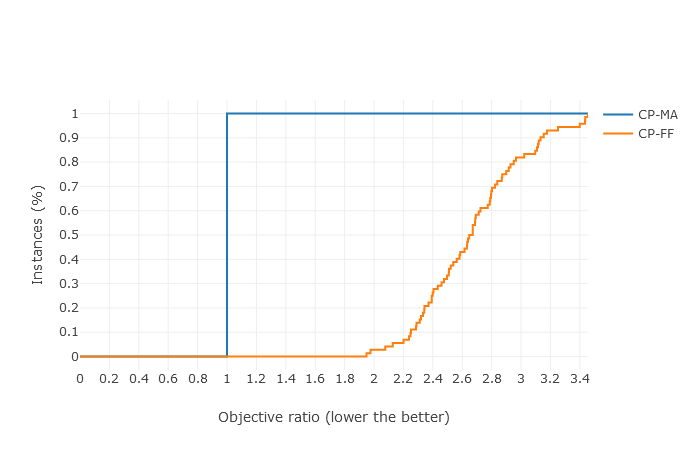
\includegraphics[scale=0.55]{experiments/heuristic.png}
  \caption{Most Available and First Fail heuristics on 72 instances (first solution).}
  \label{experiments:heuristic1}
\end{figure}

\subsection{Large Neighborhood Search}


\section{Comparing Solvers}

We now start by comparing different solvers together. \autoref{experiments:solvers:3} 
shows a performance profile generated from 216 instances of various sizes.
This benchmark was set to a time limit of 30s per instance. The baseline of this 
profile is the CP solver. We observe that the CP solver performs better than MIP in more than 80\% of instances.
However, we also tested the MIP solver by giving it a first solution obtained from CP, we can see that it slightly outperforms CP and MIP in 80\% of instances.

\begin{figure}
  \centering
  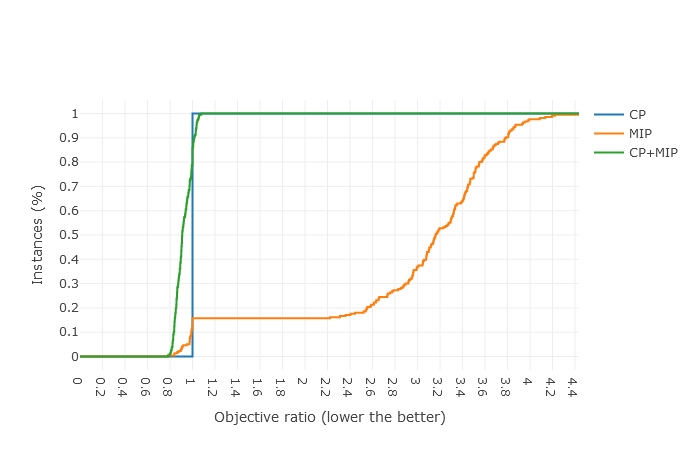
\includegraphics[scale=0.55]{experiments/solvers.png}
  \caption{CP, MIP and CP+MIP solvers on 216 instances (30s).}
  \label{experiments:solvers:3}
\end{figure}



\end{document}

